Cost is measured wall-clock latency of the GBM NumPy update kernel, on the same pre-generated coupled Brownian paths after warm-up (10,000 paths; median of 7 timings). The common target is terminal $L^1$ error at most $0.25$ currency units. We select the coarsest tested grid whose upper pointwise 95\% error interval is below this target; the actual errors need not be identical, and the tolerance overshoot is reported.\par
\begin{table}[H]\centering\small
\caption{GBM kernel costs at the common accuracy target. Both methods satisfy the same threshold; their measured errors and intervals are shown rather than assumed equal.}
\label{tab:matched-cost}\begin{tabular}{lrrrr}\toprule
Method & $N$ & Error & 95\% error CI & Median cost [ms]\\\midrule
EM & 512 & 0.23566 & [0.23177, 0.23956] & 8.532\\
Milstein & 6 & 0.21605 & [0.21087, 0.22123] & 0.139\\
\bottomrule\end{tabular}\end{table}
\begin{figure}[H]\centering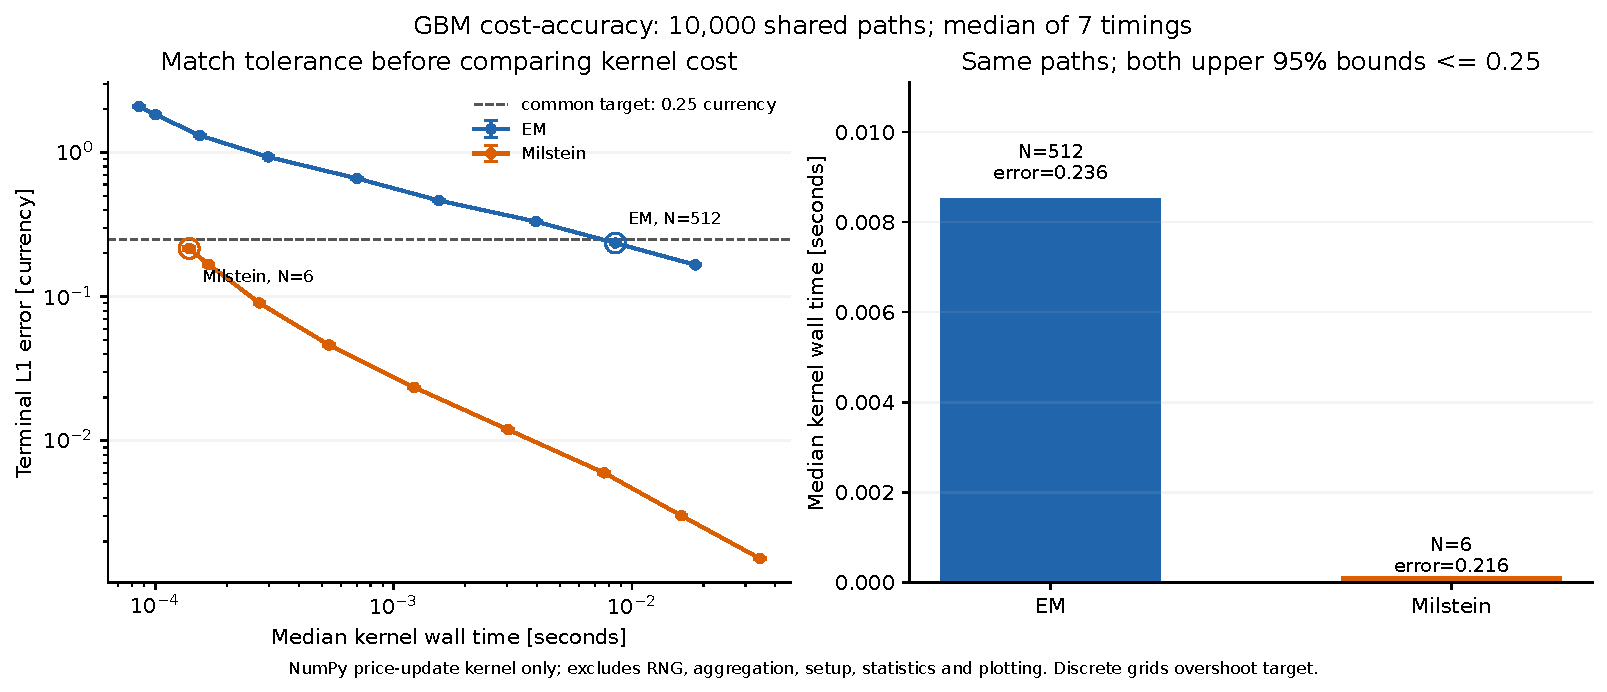
\includegraphics[width=.93\textwidth]{submission_cost_accuracy.pdf}
\caption{Measured kernel cost versus terminal strong error, using the same accuracy target and coupled paths. The target line prevents interpreting a cheap but inaccurate grid as a successful comparison.}\label{fig:cost}\end{figure}
Temporary allocations inside the price-update kernel are counted. Random-number generation, Brownian aggregation, input preparation, import/setup, compilation, statistical summaries, pilot fitting, verification and plotting are excluded from this kernel-only measure and treated consistently across methods. Raw repeated timings and the tested environment are recorded in \texttt{results/submission\_experiments.json}. The comparison in Table~\ref{tab:matched-cost} and Figure~\ref{fig:cost} therefore supports a specific implementation-level cost--accuracy conclusion, not an end-to-end runtime or cross-machine speedup.

